% 图 6.26 圆形颗粒的三种磁化组态：(a)单畴 (b)立方各向异性封闭组态 (c)单轴双畴
\documentclass[tikz,border=5pt]{standalone}
\usetikzlibrary{arrows.meta}
\usepackage{amsmath}
\usepackage{bm}
\usepackage{fontspec}
\setmainfont{Times New Roman}
\begin{document}
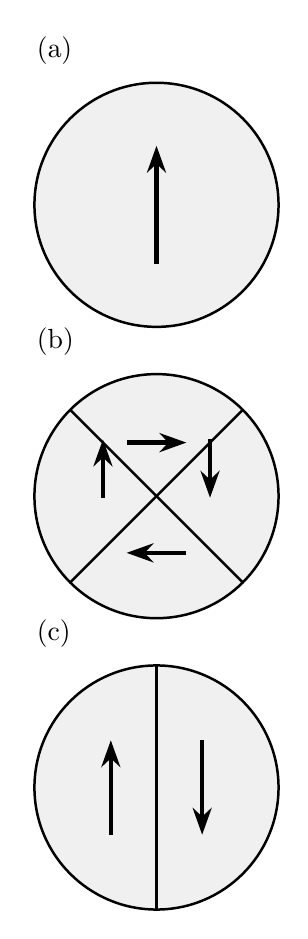
\begin{tikzpicture}[line width=0.8pt,>=Stealth,
  mag/.style={->,line width=1.6pt,>={Stealth[length=3.4mm,width=2.4mm]}}]
% ---------- (a) single domain ----------
\draw[fill=gray!12,line width=0.9pt] (1.7,11.3) circle (1.55);
\draw[mag] (1.7,10.55) -- (1.7,12.05);
\node[anchor=south west] at (0.05,12.95) {(a)};
% ---------- (b) cubic anisotropy closure configuration ----------
\begin{scope}[shift={(0,-3.7)}]
  \draw[fill=gray!12,line width=0.9pt] (1.7,11.3) circle (1.55);
  \draw[line width=0.9pt] (0.60,10.20) -- (2.80,12.40);
  \draw[line width=0.9pt] (0.60,12.40) -- (2.80,10.20);
  \draw[mag] (1.32,11.98) -- (2.08,11.98);   % top: right
  \draw[mag] (1.02,11.28) -- (1.02,12.02);   % left: up
  \draw[mag] (2.38,12.02) -- (2.38,11.28);   % right: down
  \draw[mag] (2.08,10.58) -- (1.32,10.58);   % bottom: left
  \node[anchor=south west] at (0.05,12.95) {(b)};
\end{scope}
% ---------- (c) uniaxial two-domain ----------
\begin{scope}[shift={(0,-7.4)}]
  \draw[fill=gray!12,line width=0.9pt] (1.7,11.3) circle (1.55);
  \draw[line width=0.9pt] (1.7,9.75) -- (1.7,12.85);
  \draw[mag] (1.12,10.7) -- (1.12,11.9);
  \draw[mag] (2.28,11.9) -- (2.28,10.7);
  \node[anchor=south west] at (0.05,12.95) {(c)};
\end{scope}
\end{tikzpicture}
\end{document}
